
% ===========================================================================
% Title:
% ---------------------------------------------------------------------------
% to create Type I fonts type "dvips -P cmz -t letter <filename>"
% ===========================================================================
\documentclass[11pt]{article}       %--- LATEX 2e base
\usepackage{latexsym}               %--- LATEX 2e base
\usepackage{tikz}
\usetikzlibrary{shapes.geometric, arrows}
\usepackage{booktabs}
\usepackage{graphicx}
\usepackage{subcaption}

%---------------- Tikz Flow D -----------------------------------------------

\tikzstyle{startstop} = [rectangle, rounded corners, minimum width=3cm, minimum height=1cm,text centered, draw=black, fill=red!30]
\tikzstyle{io} = [trapezium, trapezium left angle=70, trapezium right angle=110, minimum width=3cm, minimum height=1cm, text centered, draw=black, fill=blue!30]
\tikzstyle{process} = [rectangle, minimum width=3cm, minimum height=1cm, text centered, text width=5cm, draw=black, fill=orange!30]
\tikzstyle{decision} = [diamond, minimum width=3cm, minimum height=1cm, text centered, draw=black, fill=green!30]
\tikzstyle{arrow} = [thick,->,>=stealth]

%---------------- Wide format -----------------------------------------------
\textwidth=6in \textheight=9in \oddsidemargin=0.25in
\evensidemargin=0.25in \topmargin=-0.5in
%--------------- Def., Theorem, Proof, etc. ---------------------------------
\newtheorem{definition}{Definition}
\newtheorem{theorem}{Theorem}
\newtheorem{lemma}{Lemma}
\newtheorem{corollary}{Corollary}
\newtheorem{property}{Property}
\newtheorem{observation}{Observation}
\newtheorem{fact}{Fact}
\usepackage{natbib}
\newenvironment{proof}           {\noindent{\bf Proof.} }%
                                 {\null\hfill$\Box$\par\medskip}
%--------------- Algorithm --------------------------------------------------
\newtheorem{algX}{Algorithm}
\newenvironment{algorithm}       {\begin{algX}\begin{em}}%
                                 {\par\noindent --- End of Algorithm ---
                                 \end{em}\end{algX}}
\newcommand{\step}[2]            {\begin{list}{}
                                  {  \setlength{\topsep}{0cm}
                                     \setlength{\partopsep}{0cm}
                                     \setlength{\leftmargin}{0.8cm}
                                     \setlength{\labelwidth}{0.7cm}
                                     \setlength{\labelsep}{0.1cm}    }
                                  \item[#1]#2    \end{list}}
                                 % usage: \begin{algorithm} \label{xyz}
                                 %        ... \step{(1)}{...} ...
                                 %        \end{algorithm}
%--------------- Figures ----------------------------------------------------
\usepackage{graphicx}

\newcommand{\includeFig}[3]      {\begin{figure}[htb] \begin{center}
                                 \includegraphics
                                 [width=4in,keepaspectratio] %comment this line to disable scaling
                                 {#2}\caption{\label{#1}#3} \end{center} \end{figure}}
                                 % usage: \includeFig{label}{file}{caption}


% ===========================================================================
\begin{document}
% ===========================================================================

% ############################################################################
% Title
% ############################################################################

\title{Parallel Genetic Algorithms on the GPU}


% ############################################################################
% Author(s) (no blank lines !)
\author{
% ############################################################################
George Savin\\
School of Computer Science\\
Carleton University\\
Ottawa, Canada K1S 5B6\\
{\em georgesavin@cmail.carleton.ca}
% ############################################################################
} % end-authors
% ############################################################################

\maketitle

% ############################################################################
% Abstract
% ############################################################################
\begin{abstract}
Genetic Algorithms are very powerful metaheuristics that have been successfully applied in  various disparate fields. While there are many sequential parts to the algorithm, a fair amount can and has been parallelized in MIMD and SIMD fashion. In this paper, we show a SIMT GPU solution to the the knapsack combinatorial problem. We do everything, including initialization of data on the device rather than the host CPU and show speed improvements across the board.
\end{abstract}

% ############################################################################
\section{Introduction} \label{intro}
% ############################################################################

Genetic algorithms are powerful metaheuristics that draw insipiration from evolutionary ideas. Through operations such as selection, cross-over and mutation, the solution space is "evolved" and more optimal results are found each iteration (generation). These algorithms are amenable to parallelization and indeed researchers have experimented with parallelizing everything from individual operators to the whole process. However, designing parallel algorithms can differ quite fundamentally given the underlying architecture. 
Empirical and experimental researchers have predominantly been the drivers of GAs, mainly as optimization tools. 
Only two main components for most GAs that are problem specific : encoding and evaluation.
Financial pattern discovery, MAX-3SAT, layout problems, ML hyperparameter selection \cite{} are but a few of the problems GPU GAs have been used to solve.

% ############################################################################
\section{Literature Review} \label{litrev}
% ############################################################################

Using GPUs to accelerate Genetic Algorithms started to take off when NVIDIA released CUDA SDK 2.0 in 2008, allowing for more general programming tasks to be parallelized.  

A first intuitive approach is to move an operator onto the GPU that can efficiently be ran in parallel, such as the fitness evaluation across a population \cite{Maitre2009-wd}. Taking this idea further, generation of chromosomes could also moved to the GPU \cite{Cavuoti2013-oy}. Unfortunately, this constant transfer between CPU and GPU at every generation slowed down the runtime, and depending on the population size, may not have even been worth it \cite{robilliard2008population}. 

To overcome this transfer slowdown, master-slave models of a binary and real coded GAs were completely ported to the GPU \cite{Debattisti2009-su, Arora2010-ds}. Each operator (tournament selection, two-point and single point crossover, bitwise XOR mutation) became separate CUDA kernels. Both the crossover and mutation kernels in these cases suffered from the possibility of having the same chromosome operated on many times, causing inefficient usage and propagation of sub-optimal solutions.

Because of the architectural and operational constraints of the GPU, such as limited shared memory and expensive global memory lookups, models that aimed to reduce global communication fared better. Inversely, these models seemed to have less overall accuracy \cite{Zheng2011-zr}, while other works found this difference non-existant \cite{jahne2016overview}. Further follow-ups to quality of solutions between models have not been explored.

Island model GAs divide populations in the hope that diversity is preserved during evolution. On a GPU, this roughly translates to thread blocks as islands, and single threads to individuals. Within a block, fast memory access and synchronisation is available. Migration between islands occurs asynchronously.
Early island model implementations \cite{Pospichal2010-lf, Van_Luong2010-mw} used global memory only for migration. They were applied to numerical and combinatorial optimisations problems with tremendous speed-ups recorded. These speed-ups unfortunately were due mainly to comparisons with poorly optimized sequential GAs \cite{Jaros2012-ni}. When compared against properly parallelized GAs on CPUs, the speed-up was more in line with expected theoretical analysis. A similar revision of speed-up was seen with newer master-slave implementations \cite{Sinha2015-dk}. Trade-offs between speed and solution quality were analyzed and associated to parameter tuning, specifically island, generation and chromosome counts \cite{Sun2019-fj}.

During this time, research looking at optimizing GA GPU representations as well as technique improvements to leverage more parallelization was taking off. Building on the island model implementations, simulated annealing was shown to provide faster convergence when replacing mutation \cite{li2017parallel}. Memory layouts were also explored, and chromosome based layouts proved to increase locality and make better usage of caches \cite{jahne2016overview}. Different encoding representations also increased convergence speed at no detriment to solution quality \cite{Pedemonte2011-zu}. 

Newer work incorporates some of these techniques, as well as developing new ones targeting Island models almost exclusively. Random seed improvement lead to a solution technique that only generates a single random seed, yet still benefits from the uniqueness and speed one would typically get by generating seeds every generation \cite{Sun2019-fj}. Another recent paper used the idea of synchronous migration intervals to improve solution quality by avoiding unintended migrations \cite{Janssen2022-kr}. This one in particular also used the idea of allocating multiple threads per individual \cite{shah2010gpu} combined with better data organization and found that their techniques provided up to 18x speedups and better solution quality compared to the original IMGAs on the same hardware.
Newer work tries to use warp granularity to represent each island and reduce thread divergence \cite{Amin2022-xd}. They also perform synchronous and asynchronous replacement, improving solution quality, dubbing it Two-Replacement Policy. Unfortunately, these interesting island model changes were not compared to any prior island model implementations.

% ############################################################################
\section{Problem Statement} \label{probstat}
% ############################################################################
Given the take-over of Island Models as the default model for genetic algorithms on the GPU, re-visiting the master-slave model last seen in \cite{Cavuoti2013-oy} is a worthwhile endeavor. It gives us the chance to contrast the differences of these approaches on new GPU architecture and to apply the CUDA design methodology ``Assess, Parallelize, Optimize, Deploy" (APOD) \cite{bradley_2012} while we improve our model. This re-exploration is the first we know of in almost a decade, and will show that the master-slave model is a worthy alternative, and arguably should be viewed as the default when first choosing to pursue a SIMT/SIMD  acceleration of a GA. 
TODO : STill update this with the fact that we are doing this on the knapsack problem
We also apply this to the binary 01 knapsack problem. It is an important combinatorial optimisation problem.

% ############################################################################
\section{Proposed Solution} \label{propsol}
% ############################################################################
Our CPU solution stays mostly faithful to the canonical Genetic Algorithm \cite{holland1984genetic}, and serves as a launching point for the APOD parallelization towards our GPU version. Figure \ref{fig:GA} is a flowchart of our implemented algorithm. There are two GPU solutions as one represents a first parallelization attempt, and a second improved version, based on APOD changes leveraging NVIDIA GPU architecture. Differences between the two will be highlighted in each of the following operators.

\begin{figure}[h]
    \centering
    \includegraphics[width=\linewidth]{Figures/Genetic Algorithm (1).png}
    \caption{The Genetic Algorithm logical path for both the CPU and GPU version. The GPU version kernalizes these steps}
    \label{fig:GA}
\end{figure}
\subsection{Encoding Schema}
A benefit of the binary knapsack is that both the genotype and phenotype representations are the same : a string of 1's and 0's indicating the presence or absence of the respective item at that index. For our problem, each 1 or 0 is represented by an integer, for a total array of length number of items. Figure \ref{fig:encoding} shows how the chromosome encoding lines up with the profit values and weight values of each item.

\begin{figure}[h]
    \centering
    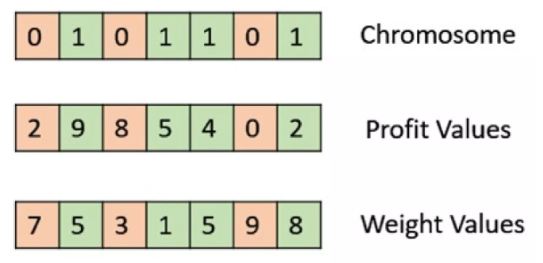
\includegraphics[width=0.5\linewidth]{Figures/knapsack_representation.png}
    \caption{Binary Knapsack chromosome encoding}
    \label{fig:encoding}
\end{figure}

\subsection{Initialization}
There are multiple ways to initialize chromosomes, and when we have a lot of items, it might make more sense to use a greedy approach, or some a priori information about the values and weights. For our own knapsack problem however, on the \textbf{CPU} we decided to use a bernoulli distribution and a mersenne twister pseudo-random generator to determine if a gene was 0 or 1. We also ensured that the total weight was not greater than the knapsack capacity by setting the remaining genes to 0 if this capacity would be crossed by a chromosome.

The \textbf{GPU} solution had to be slightly modified as none of these were readily available, and we had to rely on the NVIDIA cuRAND\footnote[1]{https://docs.nvidia.com/cuda/curand/index.html} library which used the \textit{XORWOW} generator. We also needed to split this step into two separate kernels \textit{initKernel} which sets a cuRAND handle for each chromosome, and the actual initialize kernel, \textit{initializeChromosomes} which sequentially iterated over genes and used a modulo to set either 0 or 1 values.

\subsection{Evaluation}
The \textbf{CPU} solution iterated over each chromosome sequentially and stored each respective score in the associated struct. A score of 1 was given to any chromosome that went over knapsack capacity.
The \textbf{GPU} evaluation was done in parallel on each chromosome in the  \textit{evaluateChromosome} kernel, and the same penalty of lowering the total score to 1 was applied. Existing reduction algorithms on the GPU (in our case to sum the scores of chromosomes) only used arrays of floats or ints, and not over structs, so we needed an additional \textit{pullScores} kernel to store this information into an array of scores that would then be reduced into a total sum by the \textit{reduce} kernel. This \textit{reduce} kernel was taken from the CUDA sample examples, and returned the summed result to the host.

A second improved GPU version leveraged a custom reduction we wrote did not need to pull scores down from the chromosome structs, and also did not move the total score back to the host. This was all done in a kernel called \textit{sumReducer}.

\subsection{Reproduction}
Reproduction is really an overarching function that relies on selection of parent chromosomes, actual cross-over/reproduction of these parents, and mutation of the resulting offspring. These steps need to be done sequentially, and this restriction applies to the GPU implementation as well. Afterwards, all the offspring are copied into the original chromosome array. The more optimized GPU implementation moves this copy into its own kernel that works at the gene level rather than the chromosome level to squeeze out more throughput.

\subsubsection{Selection}
Selecting parents were done by a roulette selection implementation that picked unique parents for crossover. All other papers reviewed overlooked this uniqueness in selection. Figure \ref{fig:roulette} visualizes this roulette concept. Spinning the wheel was simply the modulo between a random number and the total score sum. We spun the wheel twice for one parent, and the second time around, the wheel was spun with the first parent removed. On the GPU, this function lived on the device, and was called at the chromosome thread level. It could not be further parallelized due to the need to select a first parent.

\begin{figure}[h]
    \centering
    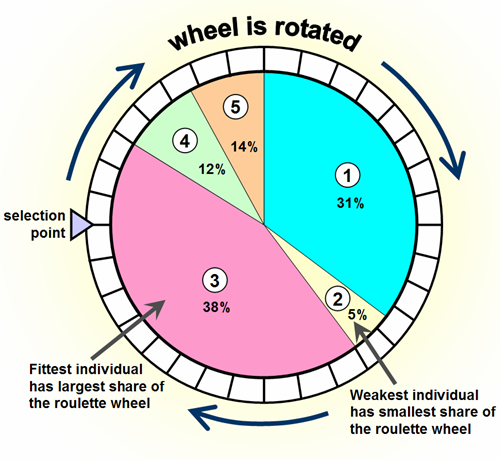
\includegraphics[width=0.5\linewidth]{Figures/roulette_selection.png}
    \caption{Roulette Selection of parent chromosomes}
    \label{fig:roulette}
\end{figure}

\subsubsection{Crossover}
The creation of offspring via crossover can be done in many ways, but for this project, we chose single point crossover. Figure \ref{fig:crossover} visualizes the single point crossover, where offspring are the parent chromosomes with swapped bits past the cutoff point. The CPU implementation allocates memory for the offspring, selects two parents and performs crossover. The GPU implementation is also at the chromosome thread level, and each thread performs this crossover, however only one of the offspring is chosen in a probabilistic manner. This was a change to ensure the algorithm would run on the GPU properly.

\begin{figure}[ht]
\begin{subfigure}{.5\textwidth}
  \centering
  % include first image
  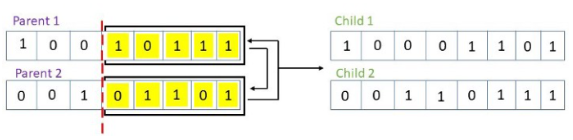
\includegraphics[width=.8\linewidth]{Figures/crossover.png}  
  \caption{Single-Point Crossover}
  \label{fig:crossover}
\end{subfigure}
\begin{subfigure}{.5\textwidth}
  \centering
  % include second image
  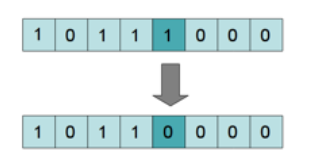
\includegraphics[width=.8\linewidth]{Figures/mutation.png}  
  \caption{Gene Mutation}
  \label{fig:mutation}
\end{subfigure}
\caption{Single point Crossover and Mutation operations}
\label{fig:cross-mutate}
\end{figure}

\subsubsection{Mutation}
Finally mutation is when a gene flips from 1 to 0, or 0 to 1. It usually has a very small probability of occurring, and in our case, we kept it at 0.001. The first GPU implementation does this in parallel at the chromosome level, whereas the second implementation does it at the thread gene level increasing throughput.

\subsection{Experiments}
Knapsack item lists of various sizes were used, along with varying population sizes to debug and test both CPU and GPU programs, however the final experiments were for a 50 item knapsack and a 1000 item knapsack. With these two sizes, population sizes ranging from 32 to 1024 were tested against all the CPU, 1st GPU implementation and post APOD 2nd GPU implementation.
NIVIDIA Nsight systems\footnote{https://developer.nvidia.com/nsight-systems} was used to profile each GPU run.

% ############################################################################
\section{Experimental Evaluation} \label{expeval}
% ############################################################################

\subsection{Hardware}
The CPU execution was done on an Intel(R) Core(TM) i7-9700K CPU @ 3.60GHz, with 32GB of RAM. The GPU used was a 12GB RTX 3060 on a Carleton cloud VM.

\subsection{Results}
\begin{figure}[h]
    \centering
    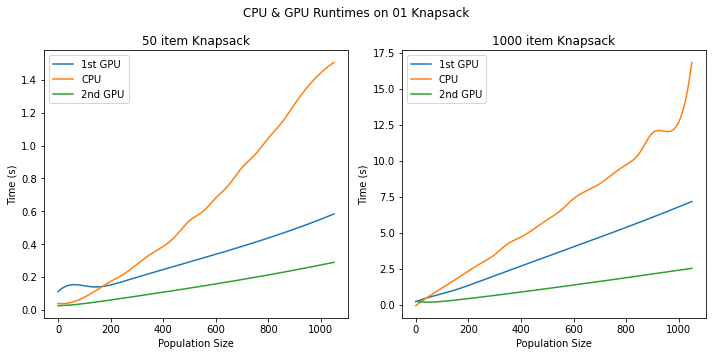
\includegraphics[width=\linewidth]{Figures/cpu_gpu_runtimes.png}
    \caption{Results of the GA for our implementations across the GPU and CPU}
    \label{fig:runtime}
\end{figure}

\begin{table}[h]
\centering
\resizebox{\textwidth}{!}{%
\begin{tabular}{@{}lllll@{}}
\toprule
Time (\%) & Total Time (ns) & Instances & Avg (ns)  & Name of Kernel          \\ \midrule
83.1      & 920,536,735     & 5,994     & 153,576.4 & GPUreproduceChromosomes \\
8.7       & 96,057,554      & 6,000     & 16,009.6  & evaluateChromosomes     \\
6.5       & 71,702,476      & 6,000     & 11,950.4  & pullScores              \\
1.4       & 15,998,624      & 6,000     & 2,666.4   & reduce                  \\
0.2       & 2,320,024       & 6         & 386,670.7 & initializeChromosomes   \\
0.1       & 1,613,520       & 6         & 268,920.0 & initKernel              \\ \bottomrule
\end{tabular}%
}
\caption{nsys profile of a 1000 generation GPU run}
\label{tab:gpu-profile}
\end{table}

\begin{table}[]
\begin{tabular}{@{}ll@{}}
\toprule
Call in Reproduction Kernel & Time (\%) \\ \midrule
Roulette Selection          & 12.2     \\
Crossover                   & 31.8     \\
Mutation                    & 56       \\ \bottomrule
\end{tabular}
\caption{The three device functions representing the majority of the work done in the reproduction kernel}
\label{tab:rep-kernel-breakdown}
\end{table}

% ############################################################################
\section{Conclusions} \label{conc}
% ############################################################################



Trying to run threads against each gene is the obvious speedup, however due to the nature of encodings and the GPU architeccture, it leads to having chromosomes split across blocks, which do not share memory and would lead to serious memory hits.
% ############################################################################
% Bibliography
% ############################################################################
\bibliographystyle{plain}
\bibliography{my-bibliography}     %loads my-bibliography.bib

% ============================================================================
\end{document}
% ============================================================================
